\documentclass[tikz]{standalone}
\begin{document}
\begin{tikzpicture}
    \node[anchor=south west,inner sep=0] at (0,0) {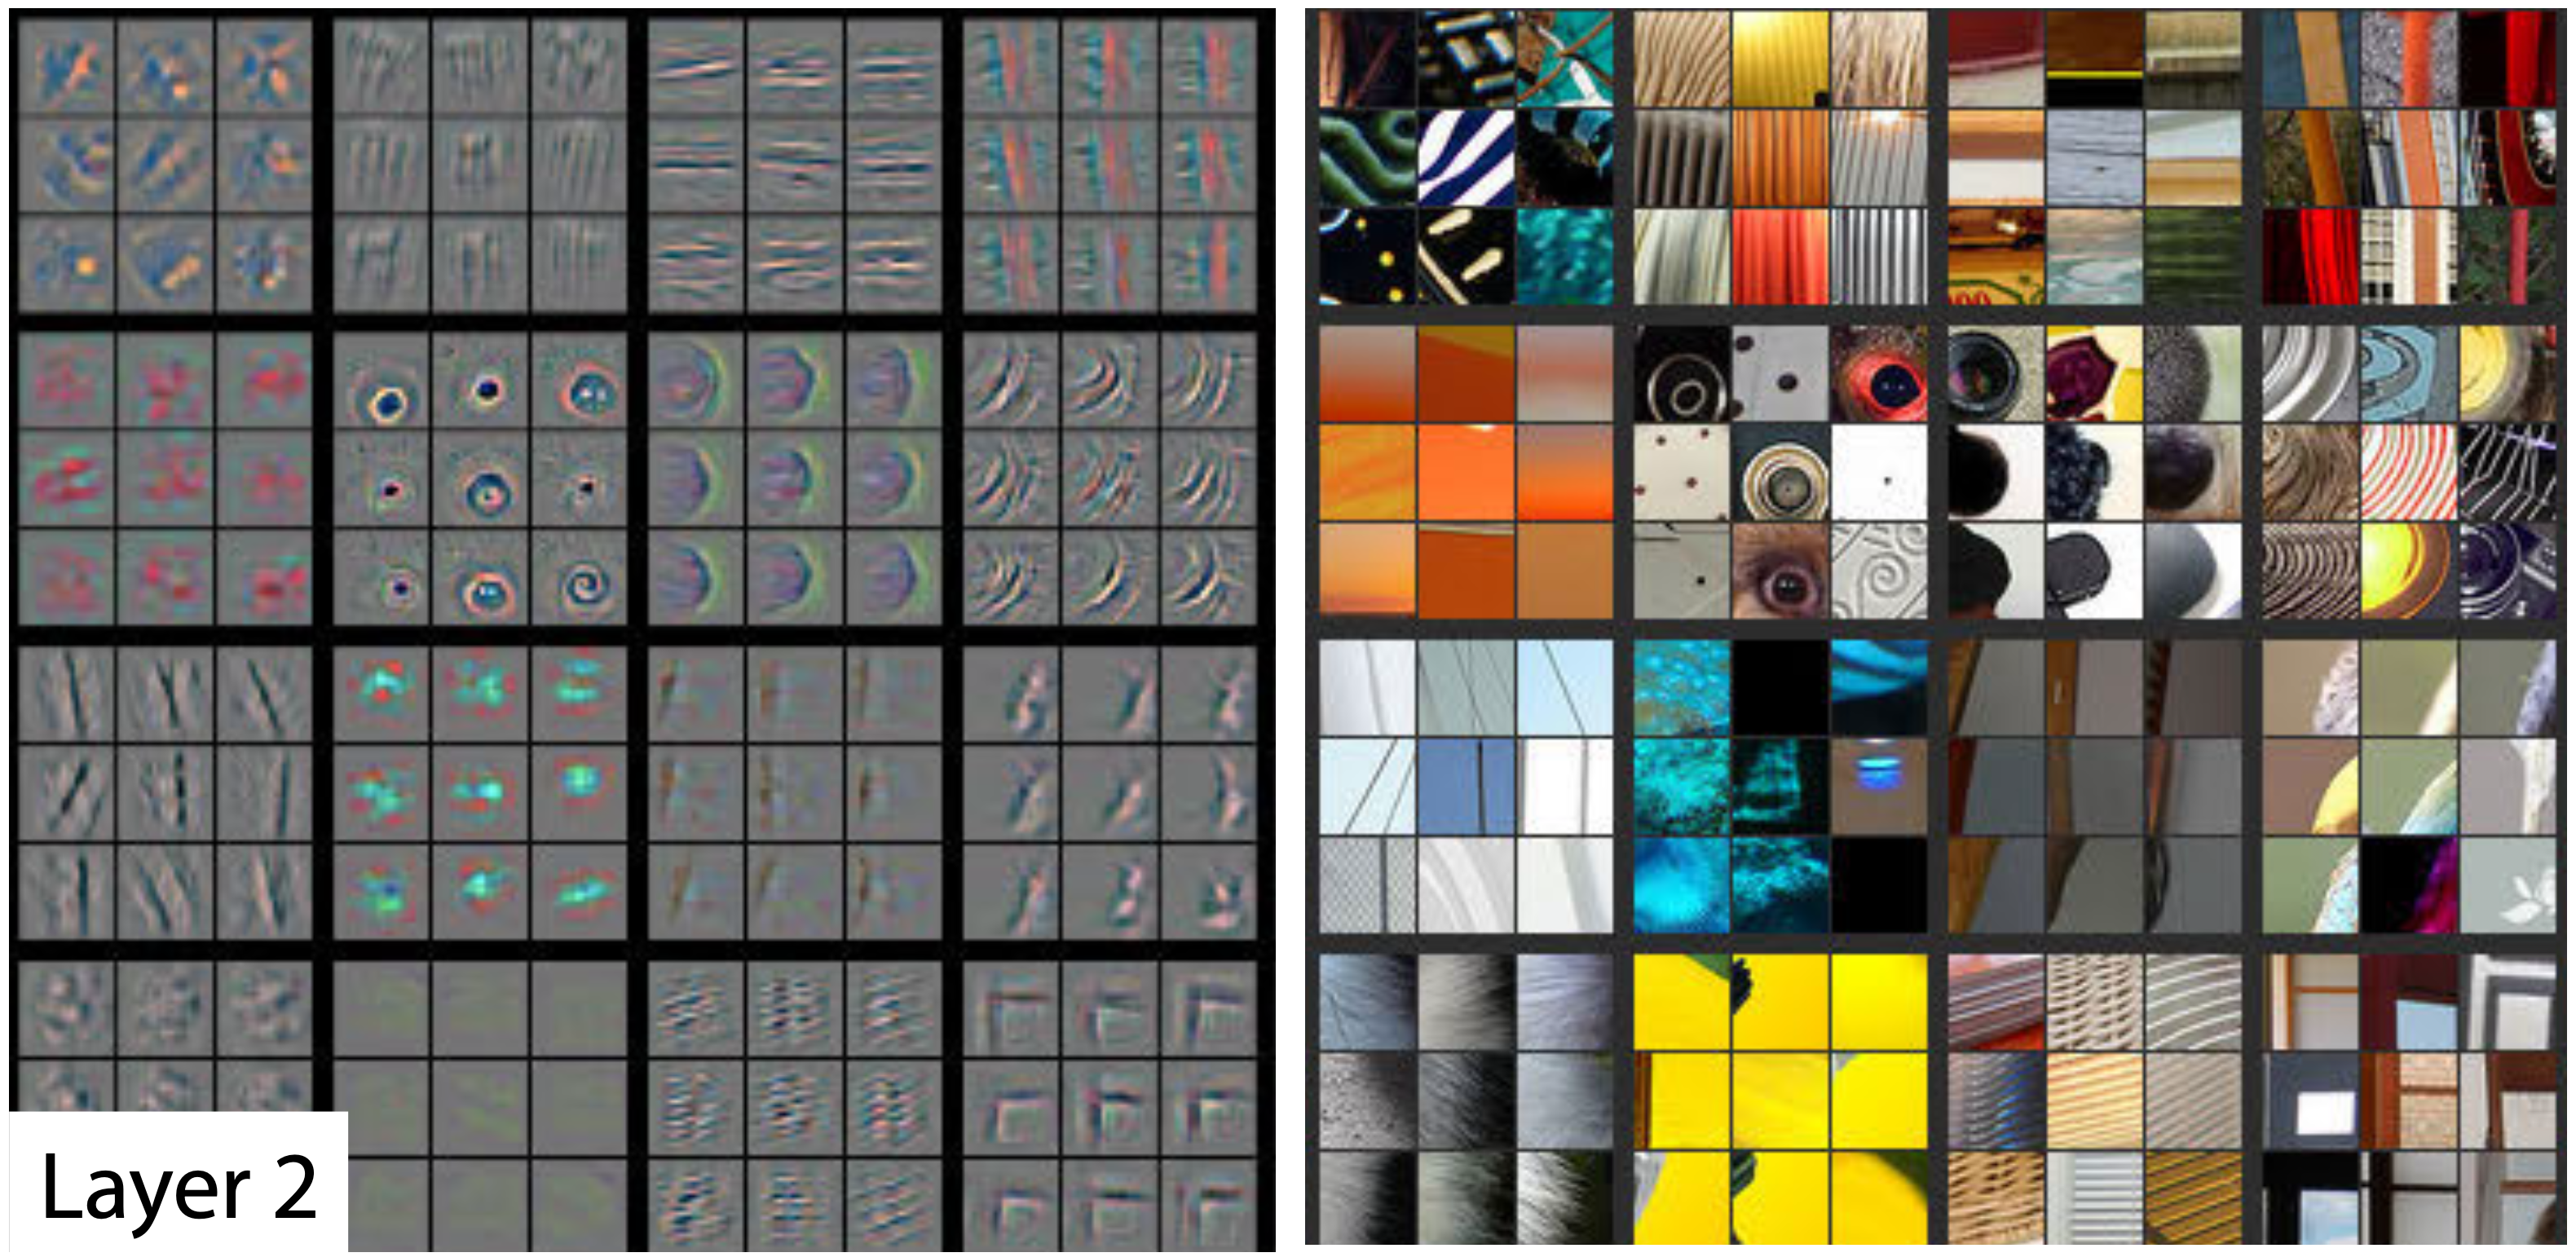
\includegraphics[width=\textwidth]{tikz/chapter5 - Deconvolutional Networks Captured Patterns Image.png}};
    \node[fill=white, anchor=south west, align=left] at (0.05,0.02) {Extracted \\ Representations};
    \draw[black, line width=2.6pt] (0.05,5.9) rectangle (6,0);
    \draw[black, line width=2.6pt] (6.15,5.9) rectangle (12.12,0);
    \draw[black, line width=2.6pt] (6.15,0.03) rectangle (12.12,0.03);
\end{tikzpicture}
\end{document}